\documentclass[english,a4paper,11pt,oneside]{memoir}

\usepackage{amsmath}
\usepackage{lipsum}
\usepackage{gensymb}
\usepackage{float}
\usepackage{wrapfig}

\newtheorem{lemma}{Lemma}

% ting til memoir
\setlrmarginsandblock{2.2cm}{*}{1}
\setulmarginsandblock{3.5cm}{*}{1}
\setheadfoot{2\onelineskip}{\footskip}
\checkandfixthelayout

% gør at subsections også nummeres
\setsecnumdepth{subsection}

\setcounter{tocdepth}{2}

%%%%%%
% ABSTRACT STYLE
%%%%%%
\makechapterstyle{abstract}{
  \renewcommand*{\printchaptername}{}
%  \renewcommand*{\chapnumfont}{\normalfont\sffamily\huge\bfseries}
  \renewcommand*{\printchapternum}{
    \flushleft
    \begin{tikzpicture}
      \draw[fill,color=black] (0,0) rectangle (2cm,2cm);
      \draw[color=white] (1cm,1cm) node { \chapnumfont\thechapter };
    \end{tikzpicture}
  }
 % \renewcommand*{\chaptitlefont}{\normalfont\sffamily\Huge\bfseries}
  \renewcommand*{\printchaptertitle}[1]{\center\chaptitlefont\Large##1}
}
%%%%%%

%%%%%%
% PAGESTYLE
%%%%%%
\makepagestyle{main}
\makepsmarks{main}{
  \createmark{chapter}      {both}{shownumber}{}{. \ }
  \createmark{section}      {both}{shownumber}{}{. \ }
  %\createmark{subsection}   {both}{shownumber}{}{. \ }
  % \createplainmark{toc}     {both}{\contentsname}
  % \createplainmark{lof}     {both}{\listfigurename}
  % \createplainmark{lot}     {both}{\listtablename}
  % \createplainmark{bib}     {both}{\bibname}
  % \createplainmark{index}   {both}{\indexname}
  % \createplainmark{glossary}{both}{\glossaryname}
}
\makeoddhead{main}{}{}{\rightmark}
\makeevenhead{main}{\leftmark}{}{}
% sidens fod: sidetal
\makeoddfoot{main}{}{}{\thepage}
\makeevenfoot{main}{\thepage}{}{}
% smid en linie under
\makeheadrule{main}{\textwidth}{\normalrulethickness}

% \setsecheadstyle{\large\bfseries\raggedright}
% \setsubsecheadstyle{\normalsize\bfseries\raggedright}

\nouppercaseheads
\pagestyle{main}
%%%%%%

%%%%%%
% CHAPTER PAGE STYLE
%%%%%%
% \makeoddhead{plain}{}{}{}
% \makeevenhead{plain}{}{}{}
% % sidens fod: sidetal
% \makeoddfoot{plain}{}{}{\thepage}
% \makeevenfoot{plain}{\thepage}{}{}
% \aliaspagestyle{chapter}{plain} % make chapter pages same page style as everything else


%%%%%%
% CHAPTER STYLE
%%%%%%
\usepackage{tikz}

\makechapterstyle{box}{
  \renewcommand*{\printchaptername}{}
%  \renewcommand*{\chapnumfont}{\normalfont\sffamily\huge\bfseries}
  \renewcommand*{\printchapternum}{
    \flushleft
    \begin{tikzpicture}
      \draw[fill,color=black] (0,0) rectangle (2cm,2cm);
      \draw[color=white] (1cm,1cm) node { \chapnumfont\thechapter };
    \end{tikzpicture}
  }
 % \renewcommand*{\chaptitlefont}{\normalfont\sffamily\Huge\bfseries}
  \renewcommand*{\printchaptertitle}[1]{\flushleft\chaptitlefont##1}
}
%%%%%%


% used for flow charts
\usetikzlibrary{shapes,arrows}
% Define block styles
\tikzstyle{decision} = [diamond, draw, fill=blue!10,
    text width=9em, text badly centered, node distance=3cm, inner sep=0pt]
\tikzstyle{block} = [rectangle, draw, fill=blue!10,
    text width=10em, text centered, rounded corners, minimum height=4em]
\tikzstyle{line} = [draw, -latex']


\usepackage[utf8]{inputenc}	%Tillader danske tegn
\usepackage[T1]{fontenc}	%Tillader danske tegn
\usepackage{graphicx}		%Tillader indsættelse af billeder
\usepackage{dcolumn}		%Bruges til at lave matematiske tabelsøjler... se datatabel
\usepackage{mathtools}		%Ekstra matematik... bare lad den være, du får muligvis brug for den.
\usepackage{siunitx}
\usepackage{microtype}
\usepackage{amssymb}
\usepackage{rotating}

\usepackage{booktabs}
\setlength{\heavyrulewidth}{0.15em}
\setlength{\lightrulewidth}{0.08em}

% Where to look for figures
\graphicspath{ {./figures/} }

\newcommand{\mc}[1]{\multicolumn{1}{c}{#1}}
%\usepackage{threeparttable}
%\usepackage{multirow}

\numberwithin{equation}{chapter}
\numberwithin{table}{chapter}
\numberwithin{figure}{chapter}
\usepackage{varioref}
\usepackage[hidelinks]{hyperref}
\usepackage[draft]{fixme}
\linespread{1.15}
\usepackage[sc]{mathpazo}
\usepackage{wasysym}
\usepackage{cite}
\usepackage{multirow}

%\newsubfloat{figure}
%\RequirePackage[caption=false,position=top]{subfig}
%\let\subtop\subfloat

\usepackage{caption}
\usepackage{subcaption}
\usepackage{graphicx}

\captionsetup[figure]{labelfont=bf, textfont={}}
\captionsetup[table]{labelfont=bf, textfont={}}

\parindent 0pt
\setlength{\parskip}{2mm plus0mm minus0mm}

% Included chapters
\includeonly{
introduction,
theory,
Techniques,
ExperimentalSetup,
results,
conclusion,
appendices
}


% Macros
\newcommand{\sref}[1]{Section~\ref{#1}}
\renewcommand{\fref}[1]{Figure~\ref{#1}}
\renewcommand{\tref}[1]{Table~\ref{#1}}
\renewcommand{\eqref}[1]{Equation~(\ref{#1})}
\renewcommand{\vec}[1]{\mathbf{#1}}
\newcommand{\half}[0]{\frac{1}{2}}
\newcommand{\mean}[1]{\ensuremath{\left\langle #1 \right\rangle}}
\newcommand{\pdiff}[2]{\frac{\partial #1}{\partial #2}} % Partial derivative
\newcommand{\ppdiff}[2]{\frac{\partial^2 #1}{\partial #2^2}} % Partial derivative
\newcommand{\mat}[1]{\ensuremath{\boldsymbol{#1}}}
\newcommand{\norm}[1]{|#1|}
\newcommand{\cov}[0]{\text{cov}}

\usepackage{listings}
\usepackage{color}
\usepackage{textcomp}
\definecolor{listinggray}{gray}{0.9}
\definecolor{lbcolor}{rgb}{1,1,1}
\lstset{
	backgroundcolor=\color{lbcolor},
	tabsize=2,
	rulecolor=,
	language=matlab,
        basicstyle=\scriptsize,
        upquote=true,
        aboveskip={1.5\baselineskip},
        columns=fixed,
        showstringspaces=false,
        extendedchars=true,
        breaklines=true,
        prebreak = \raisebox{0ex}[0ex][0ex]{\ensuremath{\hookleftarrow}},
        frame=single,
        showtabs=false,
        showspaces=false,
        showstringspaces=false,
        identifierstyle=\ttfamily,
        keywordstyle=\color[rgb]{0,0,1},
        commentstyle=\color[rgb]{0.133,0.545,0.133},
        stringstyle=\color[rgb]{0.627,0.126,0.941},
}

%%%%% BEGIN DOCUMENT %%%%%
\begin{document}
\pagenumbering{roman}
\pagestyle{plain}
%% BOS FORSIDESKABELON

\begin{titlingpage}

\begin{center}

\vspace*{0cm}
\huge
\textsc{Hydrogenation of graphene on I}r\textsc{(111) by vibrationally excited molecules}\\
\vspace{1.5cm}

\vspace{3cm}

\includegraphics[width=\textwidth]{inano_logo}
\vspace{4cm}

\large
{
    Anders Christian Løchte Jørgensen\\
    iNano, Aarhus University
}

\vspace{1.5cm}

{
  Supervisor:\\
  Liv Hornekær\\
  Department of Physics and Astronomy, Aarhus University
}

\vspace{1.5cm}
{June 2016}\\


\end{center}

%\newpage

%%%%%
% The back of the frontpage
%%%%%
%colophon

\end{titlingpage}

\setcounter{page}{3}
\chapterstyle{abstract}
\vspace{6cm}
\chapter*{Abstract}
\chapterstyle{box}

\newpage\thispagestyle{empty}\mbox{}\newpage
\tableofcontents*
%\newpage\thispagestyle{empty}\mbox{}\newpage
\newpage
\pagenumbering{arabic}
\setcounter{page}{1}
\pagestyle{main}

%%%%% INCLUDE CONTENT FILES %%%%%

%\include{filename}
\chapter{Introduction}

\chapter{Graphene}

\section{Graphene}

Graphene is a two dimensional honeycomb lattice of carbon atoms. Each carbon atom is $sp^2$ hybridized where one $s$ orbital and two $p$ orbitals form three planar bonds with a separation angle of 120\degree. The distance between the individual carbon atoms is 1.42 Å. Due to the flexibility of the $sp^2$ bonds in the z direction, many other structures can be formed by a sheet of graphene, such as fullerenes, carbon nanotubes, and graphite. The graphene unit cell consists of only two lattice points, and the lattice vectors can be written as the following:

\begin{align*}
  a_1 = \frac{a}{2}(3,-\sqrt{3}) \; a_2 = \frac{a}{2}(3,\sqrt{3})
\end{align*}

\section{Graphene on Ir}

As a monolayer of graphene is synthesized on top of a metal surface the underlying metal and the graphene monolayer rarely has identical lattice parameters. This causes a mismatch between the two layers and these will be rotated at an angle compared to each other. A moiré superstructure appears when this surface is examined by STM, because certain areas has carbon directly above iridium, and certain areas has carbon and iridum perfectly out of phase. Below, figure \ref{moireunitcell} shows the the graphene-iridium moiré unit cell.

\begin{figure}
  \centering
  \begin{subfigure}[b]{0.3\textwidth}
       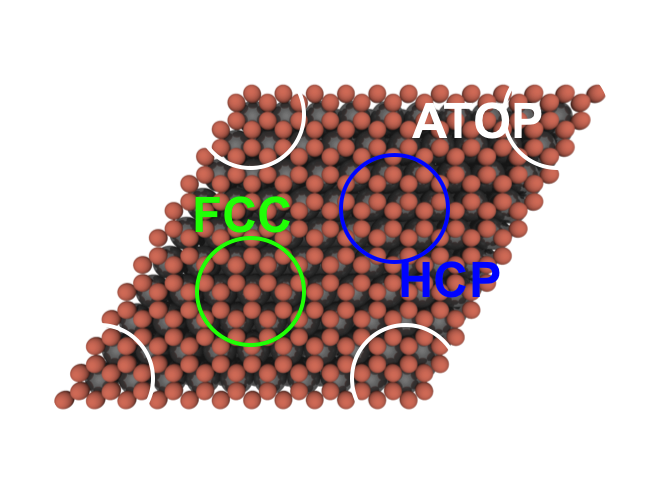
\includegraphics[width=\textwidth]{grirmoire}
       \caption{}
       \label{fig:unmarked}
   \end{subfigure}
   \begin{subfigure}[b]{0.3\textwidth}
        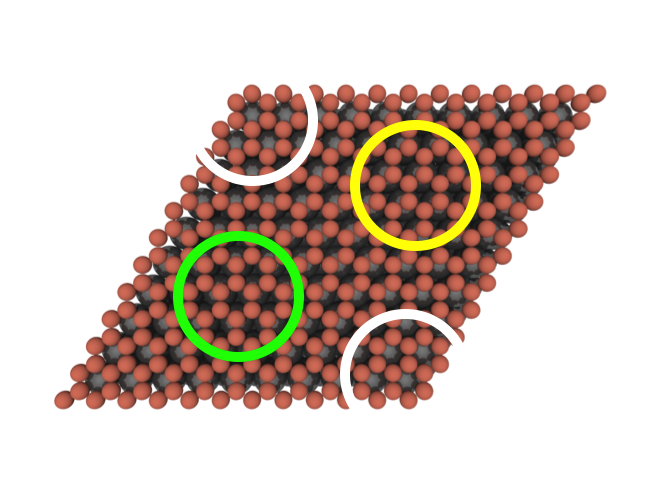
\includegraphics[width=\textwidth]{grirmoiremarked}
        \caption{}
        \label{fig:marked}
    \end{subfigure}
  \caption{Graphical interpretation of the Gr/Ir moire unit cell. \cite{Line}}
  \label{moireunitcell}
\end{figure}


\section{Hydrogenation of graphene using vibrationally excited deuterium}


\section{Hydrogenation of graphene using atomic deuterium}

\chapter{Techniques}

\section{Scanning Tunneling Microscopy - STM}

The main technique used in this study is STM, and more specifically the Aarhus STM. The working principle of the STM is the tunneling transmittivity which depends exponentially on the distance between a sharp tip and the sample. A bias is applied between the sample and the tip, and at relatively large distances the barrier that the electrons perceive is too high, and no tunneling occurs. As the distance between the sample and the tip is reduced the probability of an electron tunneling through the vacuum barrier increases until a point where tunneling happens, and the current can be measured. The tunneling current is reduced by about a factor of 10 for every ångstrøm.\cite{STMbinnig} This ensures that the STM is a very precise technique and hence essential for surface scientists. In order to achieve the tunneling current it is necessary that the tip as well as the sample is conducting.\\
In order to create an image, the surface of the sample is scanned with the tip, which is moved by piezo-elements. The tunneling current is dependant on distance between tip and sample as well as the local density of states (LDOS). A map of the LDOS is therefore obtained when the tip is scanned across the surface of the sample. This is used to indirectly create an image of the surface.\\


\section{Temperature Programmed Desorption - TPD}



\section{Low Energy Electron Diffraction - LEED}



\section{Raman Spectroscopy}

\chapter{Experimental Approach}
\label{cha:procedure}

\section{The Coal Chamber}

  The experiments are carried out under UHV (ultra high vacuum) conditions. This is crucial because contaminants easily can adsorb to the surface which ruins the quality of the gathered data. During this project the vacuum chamber named 'The Coal Chamber' is used which is one of many vacuum chambers in the SDL lab.\\
  The equipment mounted on The Coal Chamber, which is used in this study, is described in the following section along with the experimental approach. The sample is introduced to the coal chamber from a loadlock where the sample is attached to a transfer arm. Transfer of the sample from the loadlock to the main chamber takes place as the pressure in the loadlock is reduced sufficiently by a turbo pump. In the main chamber a manipulator is apparent in the center from where the sample can be transferred to the STM by a wobble stick. A filament lies behind the sample in the manipulator, which is used during anneals.

% \subsection{Turbo pump}
%
%  In order to achieve proper UHV conditions a turbo pump is needed in addition to the roughing pump. The turbo pump is directly connected to the vacuum chamber and consists of a series of rotor blades. Each of these adds momentum to the remaining gas molecules that collide with the blades and hence removes these from the chamber. In order to function properly these rotor blades spins up to 80.000 RPM.\cite{hofTurbo}

\section{STM imaging and D$_2$ dosage}

The STM was used to get a visualization of the coverage of hydrogen on the sample surface, and to analyse the sample between the different experiments.


write things about linescans, calibration and FFT/noise removal.

\section{TPD}

A mass spec is connected to the UHV chamber, and this was used to investigate the desorption of deuterium from the sample surface. The sample was positioned in the manipulator as the experiments were carried out. From here the nozzle of the mass spec was brought within millimeters of the sample. The temperature was logged together with the amount of deuterium detected by the mass spec. The mass spec was set to count masses of 4 amu, in order to exclude other molecules than deuterium. This setup was made with the computer program 'MASsoft' by Hiden Analytical.\\
A Eurotherm 2704 controller was used to control the current going to the filament in the manipulator, in order to manage the temperature of the sample. The controller was programmed to ramp the sample temperature from 300K to 900K at a rate of 1K per second. At maximum temperature the eurotherm was set to rest for 30s, and then slowly decrease the temperature to a final temperature of 300K. This cycle was performed each time a TPD measurement was carried out. During this procedure most of the deuterium on the surface should be desorped from the sample.\\
\begin{align*}
  T_{surface} = T_{TC} * 0.7921 + 131.2
\end{align*}
\begin{figure}
  \centering
  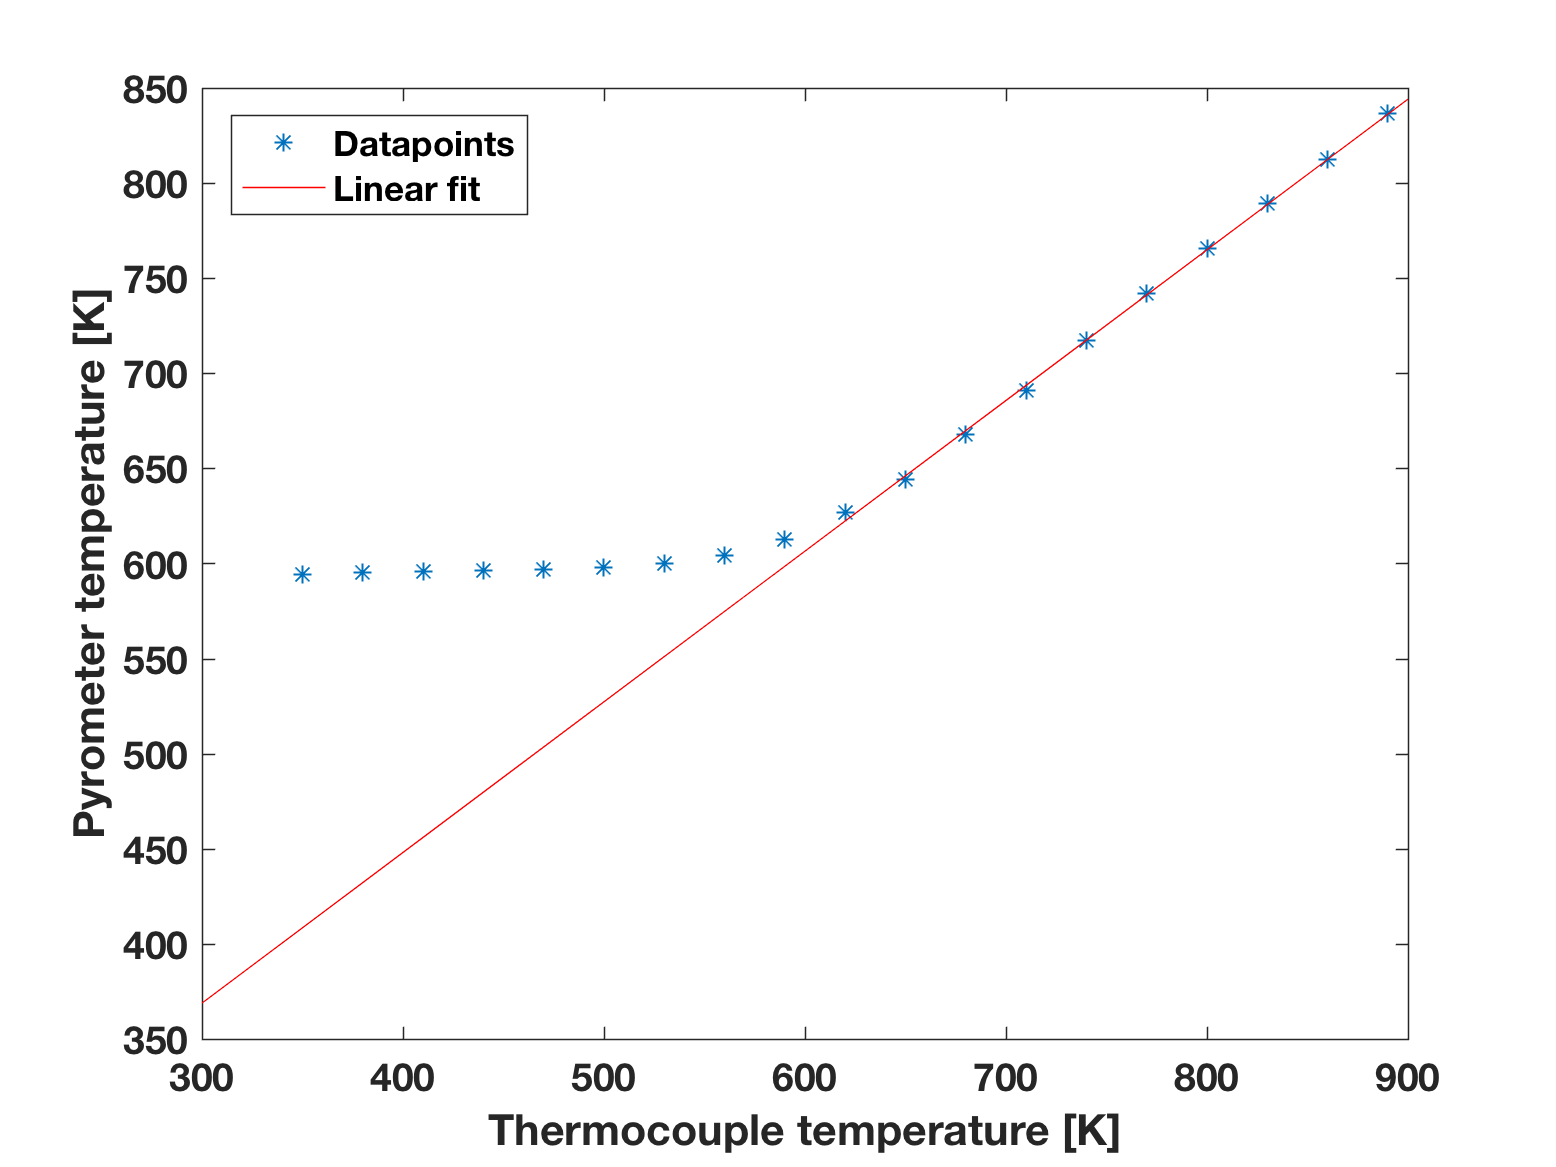
\includegraphics[width=0.55\textwidth]{TPD/kalibrering}
  \caption{Calibration of the temperature during the TPD measurements. The temperature of the surface measured by an optical pyrometer is plotted against the thermocouple temperature.}
  \label{TPDcalibration}
\end{figure}
In figure \ref{TPD:example} the data obtained from a typical TPD measurement is shown. Since the desorption of D$_2$ from the surface is investigated, a mass of 4 amu is monitored along with the temperature. It is seen that the temperature follows has a linear ramp except for the extremities of the temperature interval where some fluctuations start to happen. A different sample of Gr/Ir was used later on in the project, where the thermocouple seemed to have a loose connection. The temperature reading from this thermocouple dropped out at some points, and seemed unstable. Since the thermocouple was changed, and a new sample holder was used, the Eurotherm controller parameters needed to be autotuned, in order to achieve a linear temperature ramp once again. This caused some problems however, and the results from one of the TPD measurements from this sample can be seen in figure \ref{TPD:fail}. It is seen on figure \ref{TPD:example2} that the temperature ramp is obviously not linear. The jumps in temperature do not seem to be systematic, which might indicate that the thermocouple as well as the controller parameters both had influence on the bad temperature ramp. The influence of the non linear ramp is also seen on the D$_2$ counts, where small peaks appear when the temperature changes rapidly. As seen on figure \ref{TPD:peak2} another peak appears right after the initial due to the jump in temperature. The initial peak was judged to reflect the desorption of hydrogen best, and hence this peak was used, as seen from the green circle. \\
Since the temperature is controlled and logged with the Eurotherm controller, it is possible to plot the counts of D$_2$ against the temperature. These plots are presented in chapter \ref{cha:results}.\\
A triple gaussian function was fitted to the datapoints around the peak, in order to determine the temperature belonging to the peak. The peak value was estimated by visual observation, and the datapoints within $\pm$60\degree C are included in the fit. The temperature at the maximum of the fit was determined, and these values are presented in chapter \ref{cha:results} as the peak temperatures. An example of the fit to the peak values is shown in figure \ref{TPD:peak}. From this figure it is seen that the temperature at which the maximum counts is observed, not necessarily corresponds to the correct peak temperature. The green circle in figure \ref{TPD:peak} shows the found peak from which the temperature was gathered.\\
In order to compare the individual peaks, the background was subtracted from every datapoint. The sample was positioned stationary in front of the nozzle for a period of time before the measurements were carried out. These datapoints were used to calculate a mean background count, which was subtracted.

\begin{figure}[H]
  \centering 
  \begin{subfigure}[b]{0.45\textwidth}
    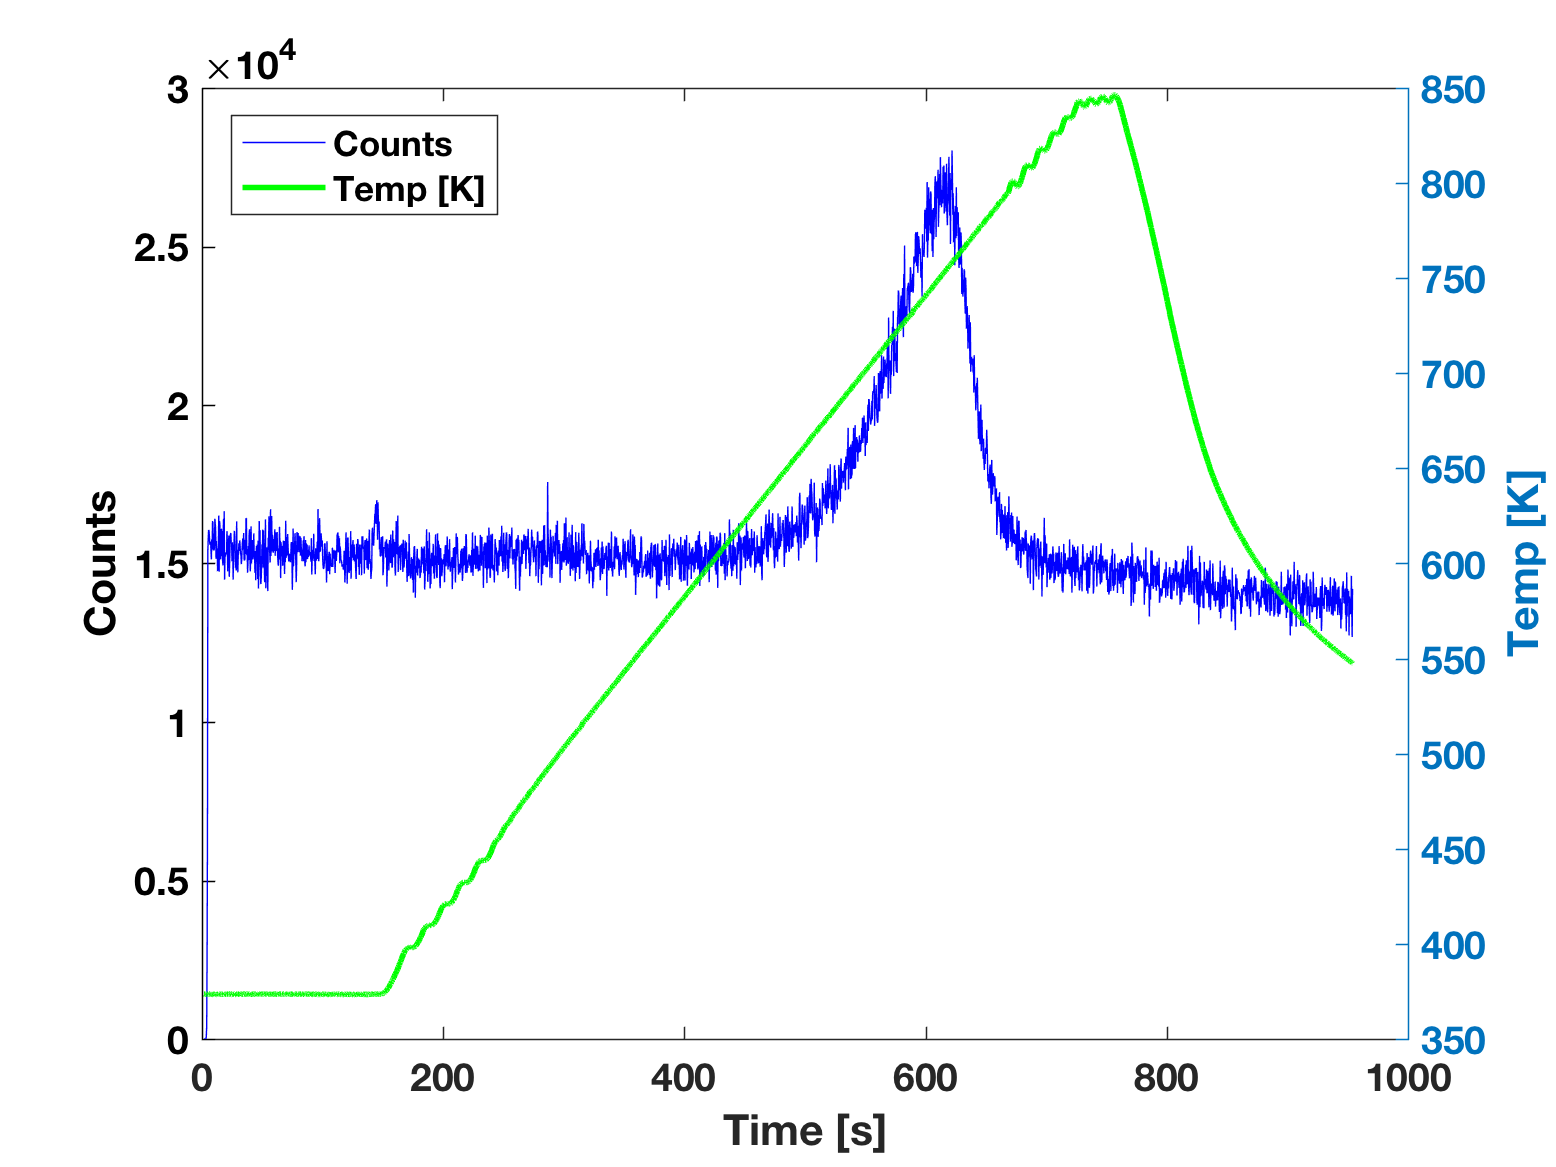
\includegraphics[width=\textwidth]{TPD/GrIr1740CD2_2504}
    \caption{}
    \label{TPD:example}
  \end{subfigure}
  \begin{subfigure}[b]{0.45\textwidth}
    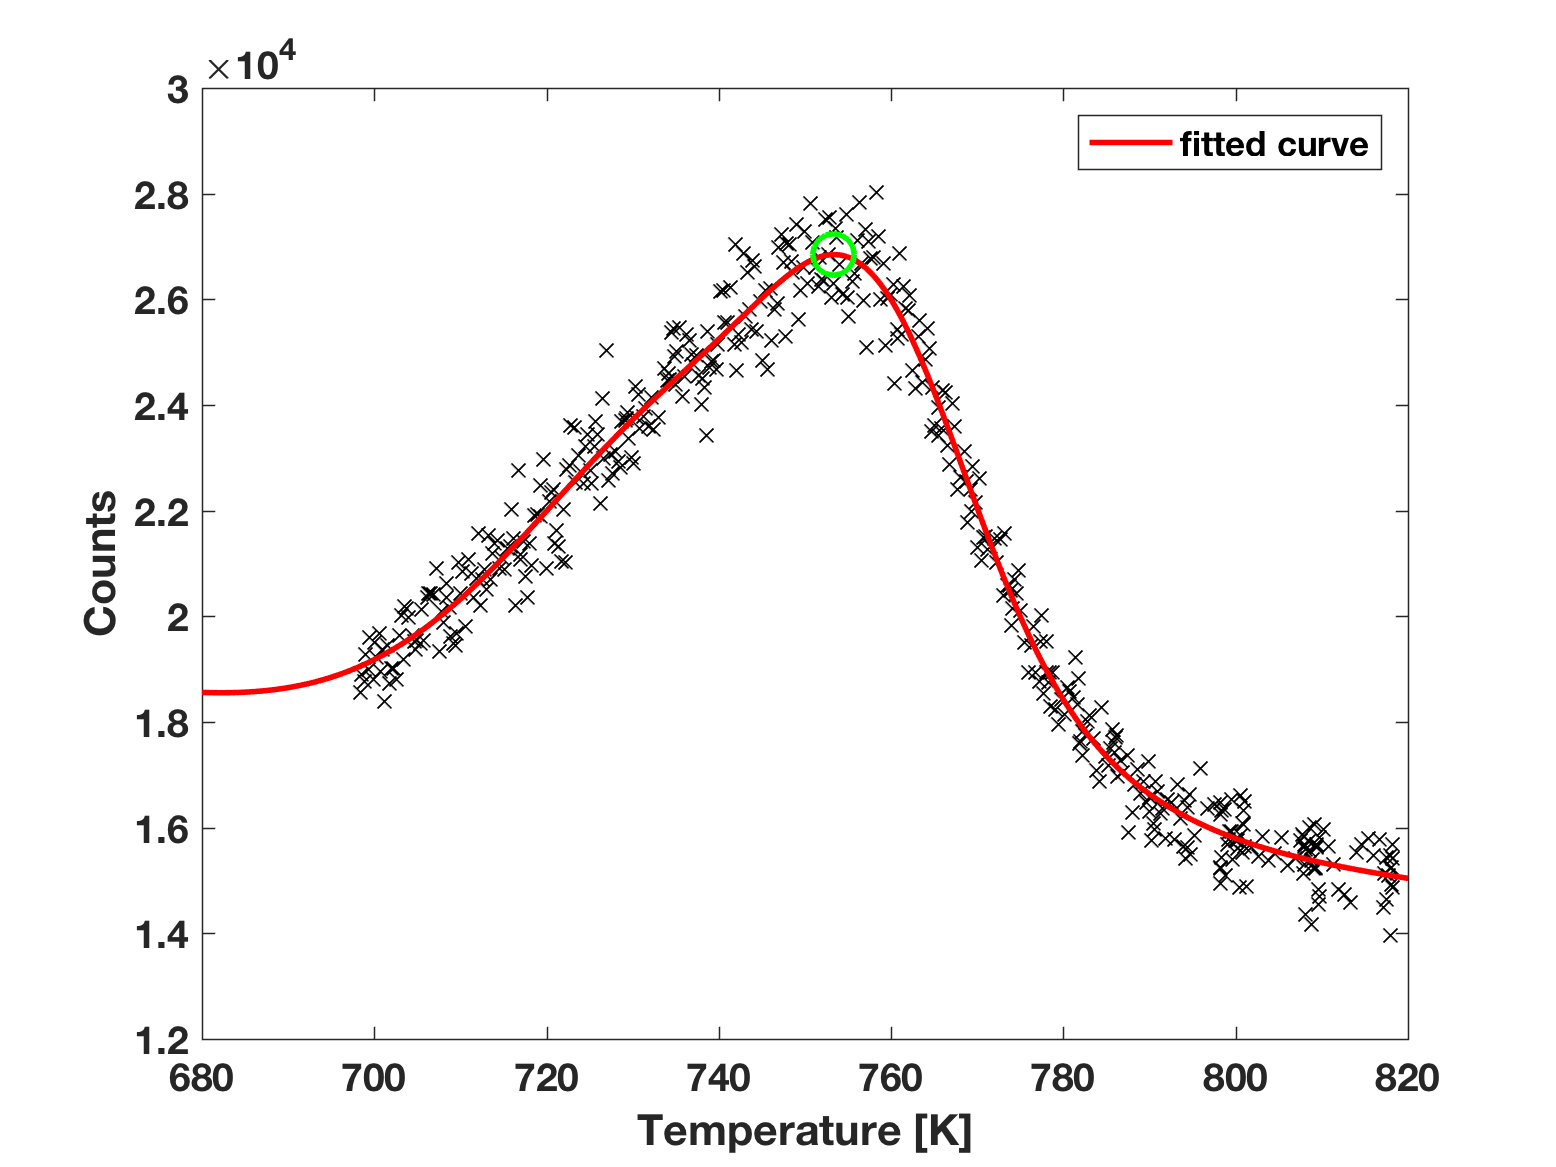
\includegraphics[width=\textwidth]{TPD/GrIr1740CD2_2504peak}
    \caption{}
    \label{TPD:peak}
  \end{subfigure}
  \caption{}
  \label{TPD:win}
\end{figure}


\begin{figure}[H]
  \centering
  \begin{subfigure}[b]{0.45\textwidth}
    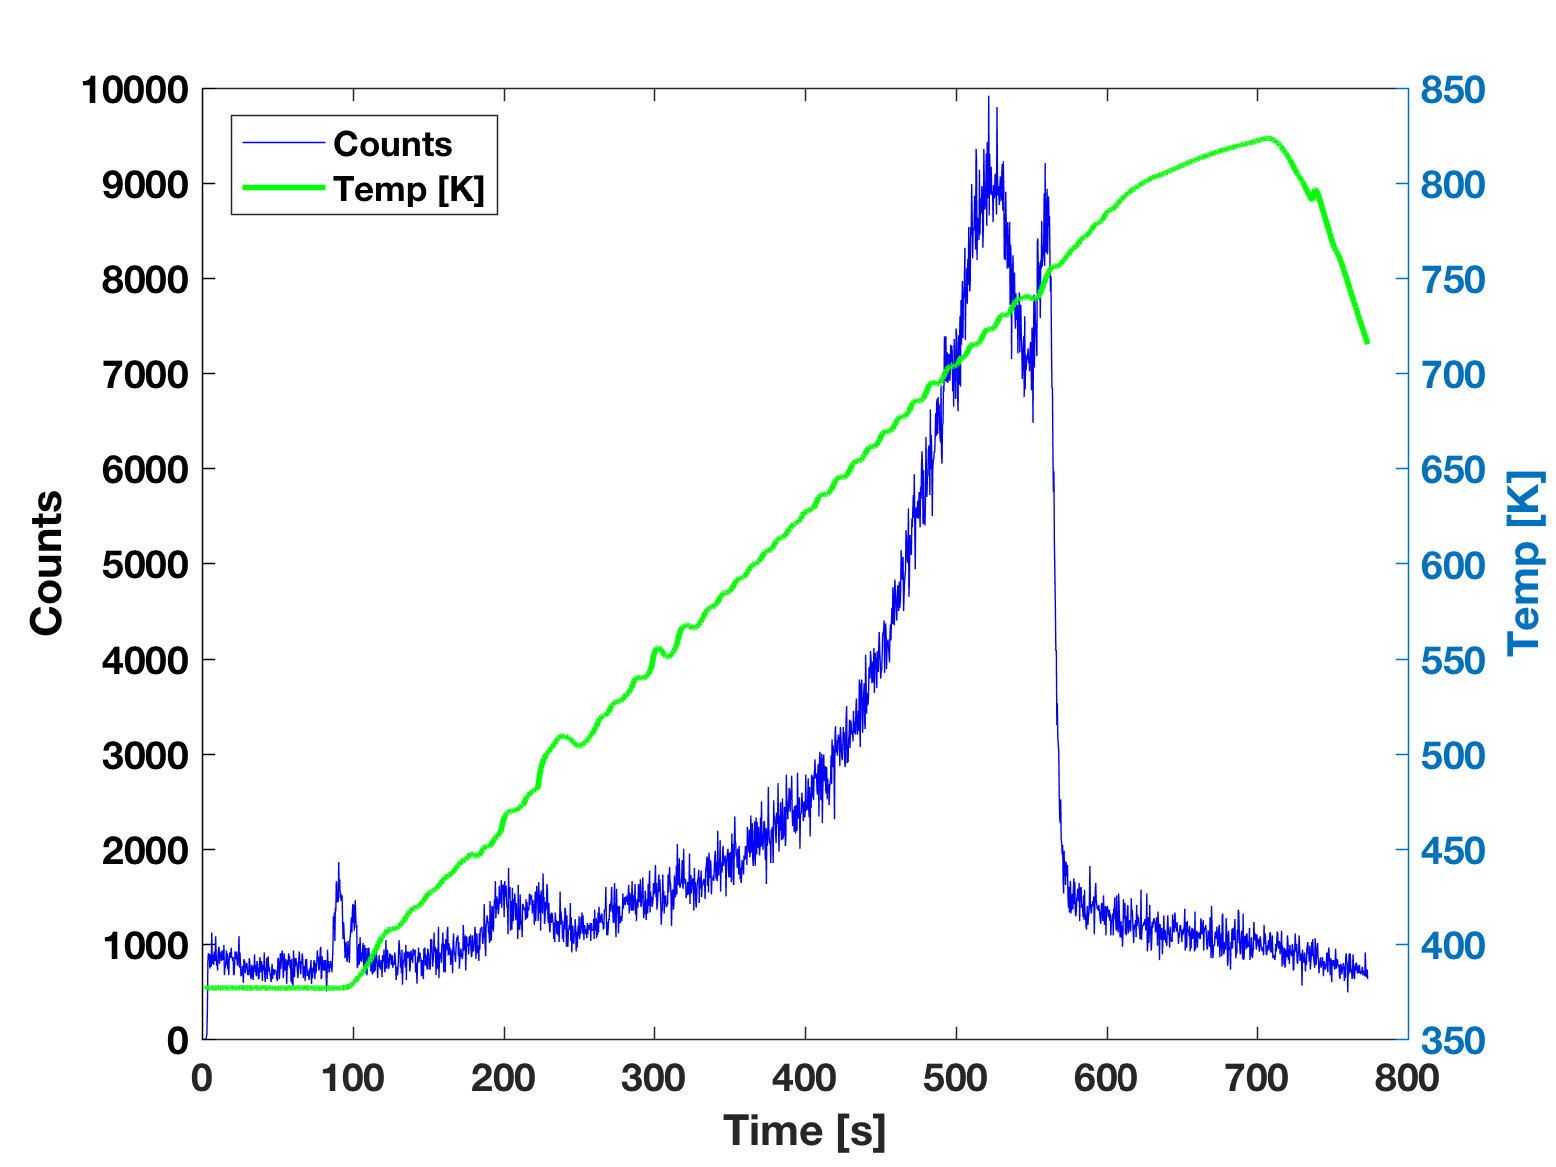
\includegraphics[width=\textwidth]{TPD/050516IrSorenD2dose1hour2}
    \caption{}
    \label{TPD:example2}
  \end{subfigure}
  \begin{subfigure}[b]{0.45\textwidth}
    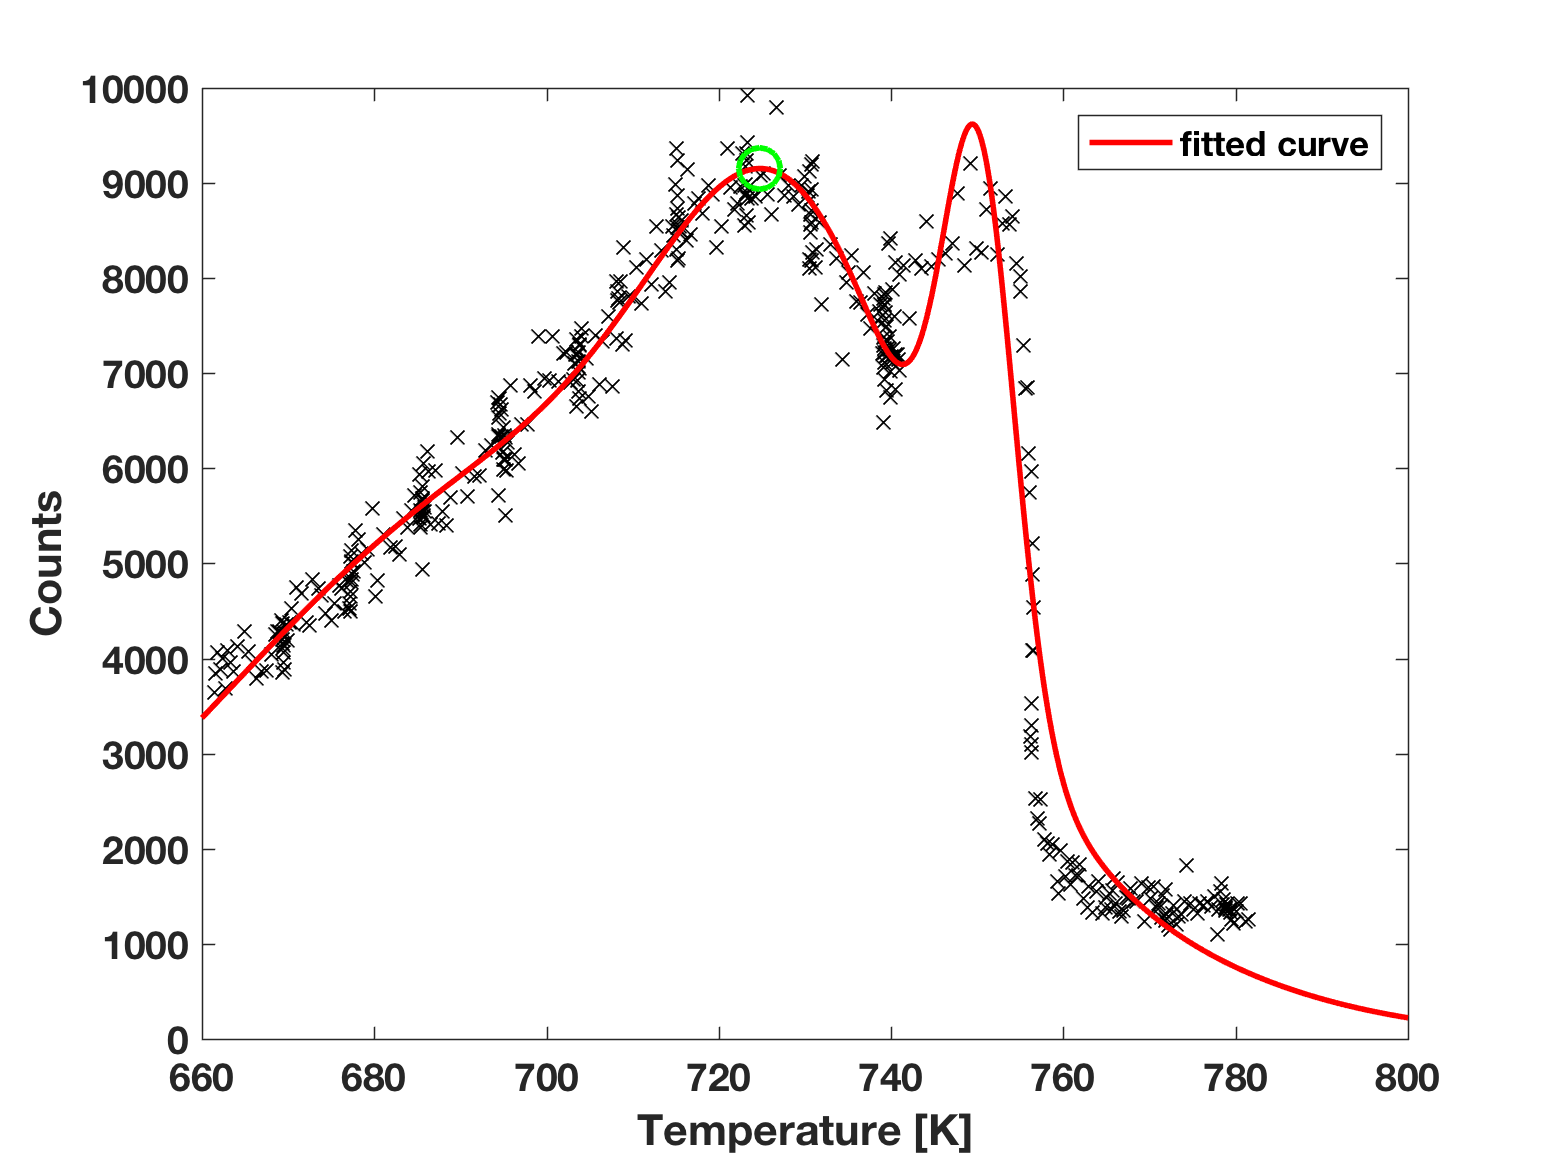
\includegraphics[width=\textwidth]{TPD/050516IrSorenD2dose1hour2peak}
    \caption{}
    \label{TPD:peak2}
  \end{subfigure}
  \caption{}
  \label{TPD:fail}
\end{figure}

\chapter{Results}
\label{cha:results}

\section{Graphene on Ir}

The quality of the graphene was checked each time D$_2$ was dosed on the sample, in order to ensure that the amount of defects was at a minimum. STM pictures of pure graphene on Ir(111) is shown in this section. On figure \ref{GrIr} pictures of graphene on Ir in different sizes is shown. Figure \ref{GrIr1} shows a large image of a graphene monolayer covering the Ir surface. Although the quality of the image is of low quality, the moire pattern is perceived. Also several step edges from the underlying Ir surface is seen. Several line scans has been performed on these edges, which show that the height difference is 2Å $\pm$0.4Å. This value is consistent with the value of 0.22nm found in the litterature.\cite{1367-2630-11-2-023006}\\
On figure \ref{GrIr2} a high resolution image of Gr/Ir is seen. The moire pattern is very prominent in this figure, and the spacing between the individual sites in the moire unit cell can be determined from a line scan. A line scan was drawn on figure \ref{GrIr2} and two points were positioned in the corners of the moire unit cell in order to obtain the moire periodicity. The morié periodicity is 25.2 $\pm$ 0.4Å according to the litterature.\cite{1367-2630-10-4-043033} This agrees with the measured length of 25.24 Å from the line scan. Typical defects on of the graphene monolayer is seen as well in this figure. Also the hexagonal pattern of graphene is sensed because of the atomic resolution. On figure \ref{GrIr3} the individual carbon atoms are even more clear.\\

\begin{figure}[H]
\makebox[\textwidth][c]{
  \begin{subfigure}[b]{0.3\paperwidth}
    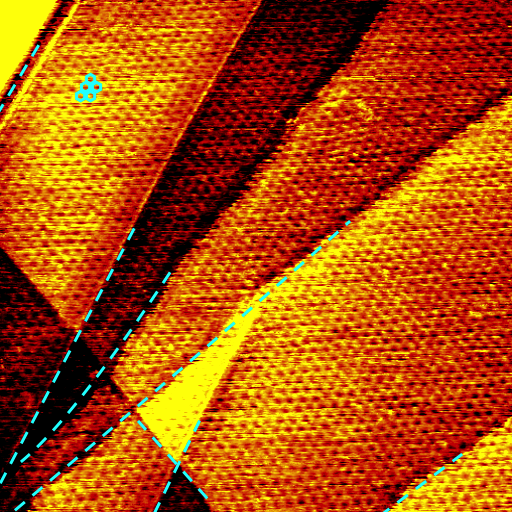
\includegraphics[height=\textwidth]{STMdata/FFT/2016-04-11_000_33.png}
    \caption{993x993 Å - 0.690 nA 78.1 mV}
    \label{GrIr1}
  \end{subfigure}
  \begin{subfigure}[b]{0.3\paperwidth}
    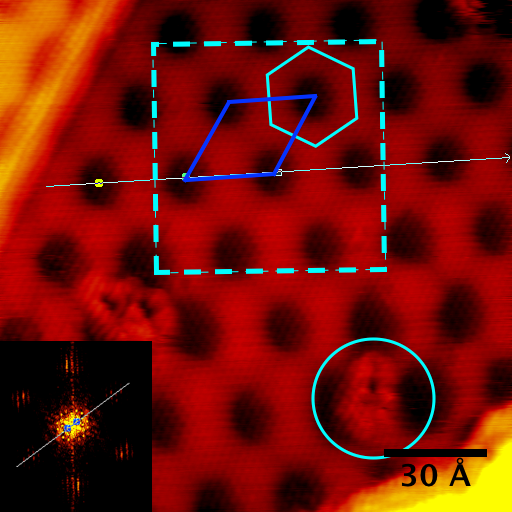
\includegraphics[height=\textwidth]{STMdata/FFT/2016-04-11_000_50.png}
    \caption{148x148 Å - -0.890 nA -311.3 mV}
    \label{GrIr2}
  \end{subfigure}
  \begin{subfigure}[b]{0.3\paperwidth}
    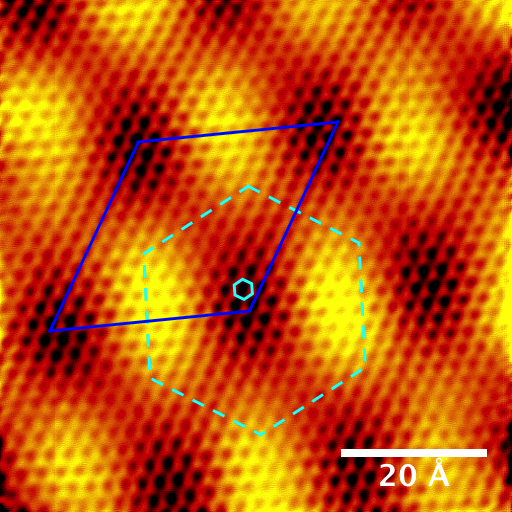
\includegraphics[height=\textwidth]{STMdata/FFT/2016-04-11_000_56.png}
    \caption{70x70 Å - 0.910 nA 311.3 mV}
    \label{GrIr3}
  \end{subfigure}
}
\caption{}
\label{GrIr}
\end{figure}

\section{D2 on graphene}

Dosing at temperatures of, 1340C, 1540C and 1740C were performed in order to determine the threshold temperature of the hydrogenation of graphene.

Full coverage D2 on graphene




1740 C doser ...

\begin{figure}[H]
\makebox[\textwidth][c]{
  \begin{subfigure}[b]{0.3\paperwidth}
    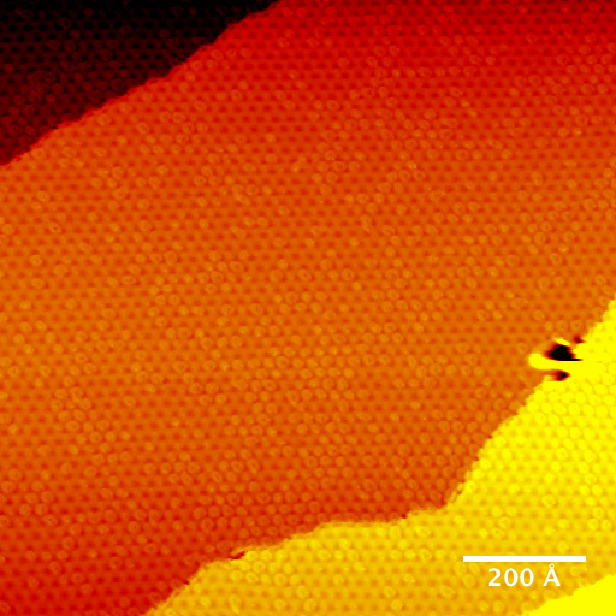
\includegraphics[height=\textwidth]{STMdata/FFT/2016-04-11_003_14.png}
    \caption{998x998 Å - 1060 nA 67.1 mV}
    \label{}
  \end{subfigure}
  \begin{subfigure}[b]{0.3\paperwidth}
    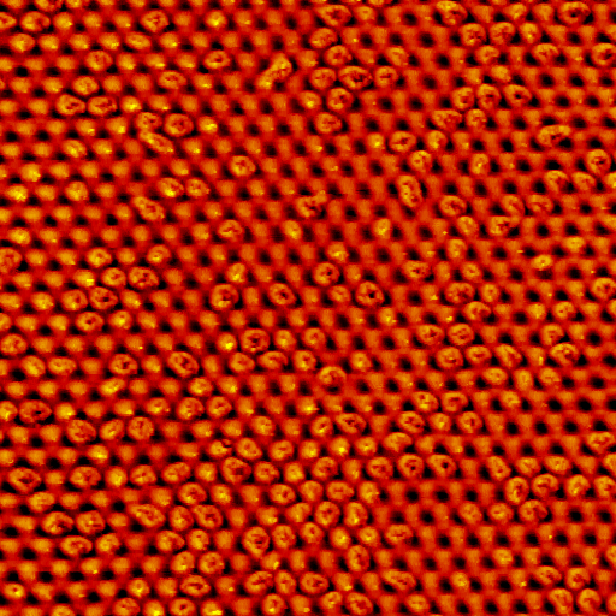
\includegraphics[height=\textwidth]{STMdata/FFT/2016-04-11_003_15.png}
    \caption{497x497 Å - 1.080 nA 67.1 mV}
    \label{}
  \end{subfigure}
  \begin{subfigure}[b]{0.3\paperwidth}
    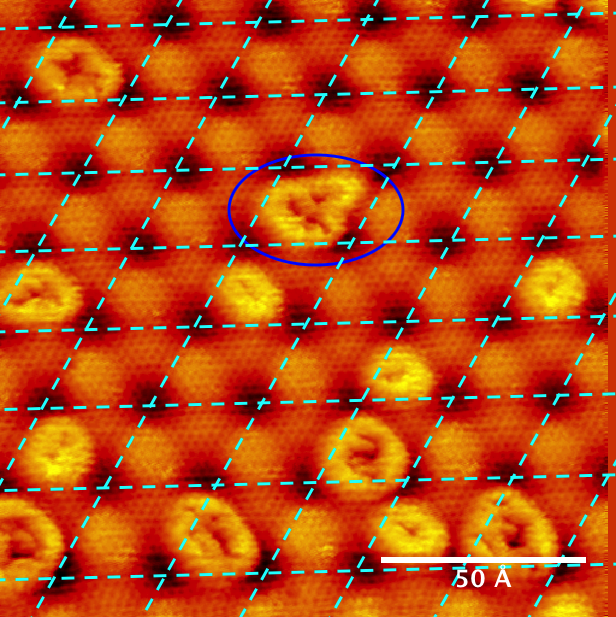
\includegraphics[height=\textwidth]{STMdata/FFT/2016-04-11_003_23.png}
    \caption{150x150 Å - 1.090 nA 67.1 mV}
    \label{}
  \end{subfigure}
}
\caption{}
\label{}
\end{figure}

1593 C doser ...

\begin{figure}[H]
\makebox[\textwidth][c]{
  \begin{subfigure}[b]{0.3\paperwidth}
    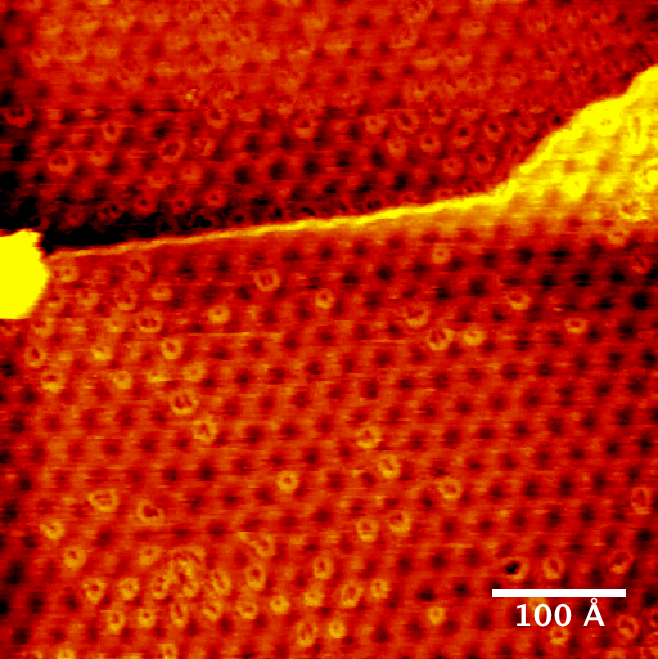
\includegraphics[height=\textwidth]{STMdata/FFT/2016-04-14_000_44.png}
    \caption{488x488 Å - 0.900 nA 190.4 mV}
    \label{}
  \end{subfigure}
  \begin{subfigure}[b]{0.3\paperwidth}
    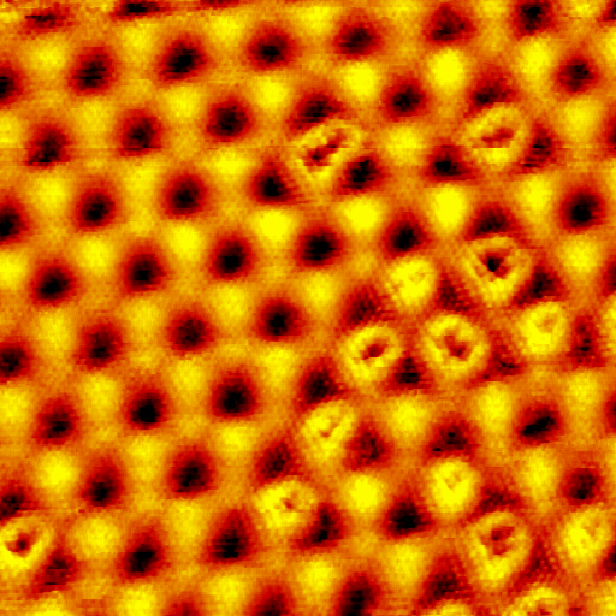
\includegraphics[height=\textwidth]{STMdata/FFT/2016-04-14_000_27.png}
    \caption{180x180Å - 1.020 nA 190.4 mV}
    \label{}
  \end{subfigure}
  \begin{subfigure}[b]{0.3\paperwidth}
    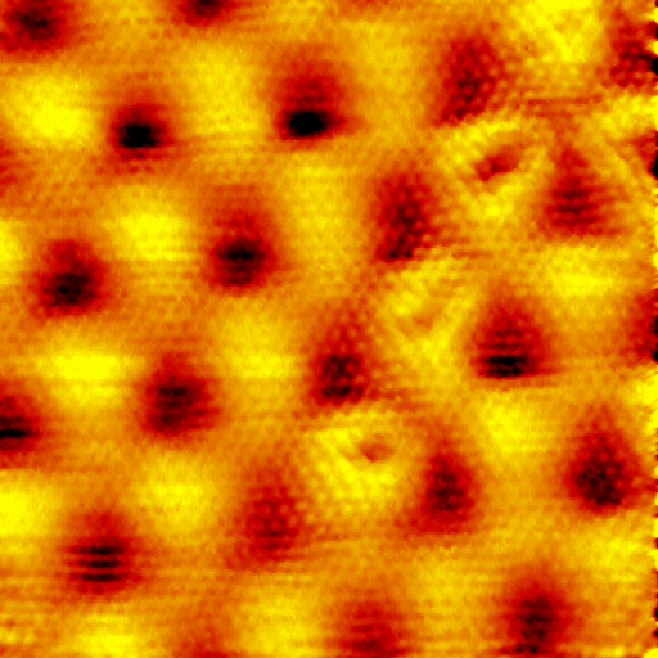
\includegraphics[height=\textwidth]{STMdata/FFT/2016-04-14_000_29.png}
    \caption{97x97 Å - 1020nA, 190.4mV}
    \label{}
  \end{subfigure}
}
\caption{}
\label{}
\end{figure}



\section{TPD measurements - Atomic and molecular D2}

In figure \ref{TPD:all} below, the data from the TPD is gathered in two different figures. TPD measurements were made for both the vibrationally excited molecules and atoms. Figure \ref{TPD:D2} shows the data aquired for the D2 dose and figure \ref{TPD:D} shows the data for the dose with hot atoms.

\begin{figure}[H]
  \centering
  \begin{subfigure}[b]{0.45\textwidth}
    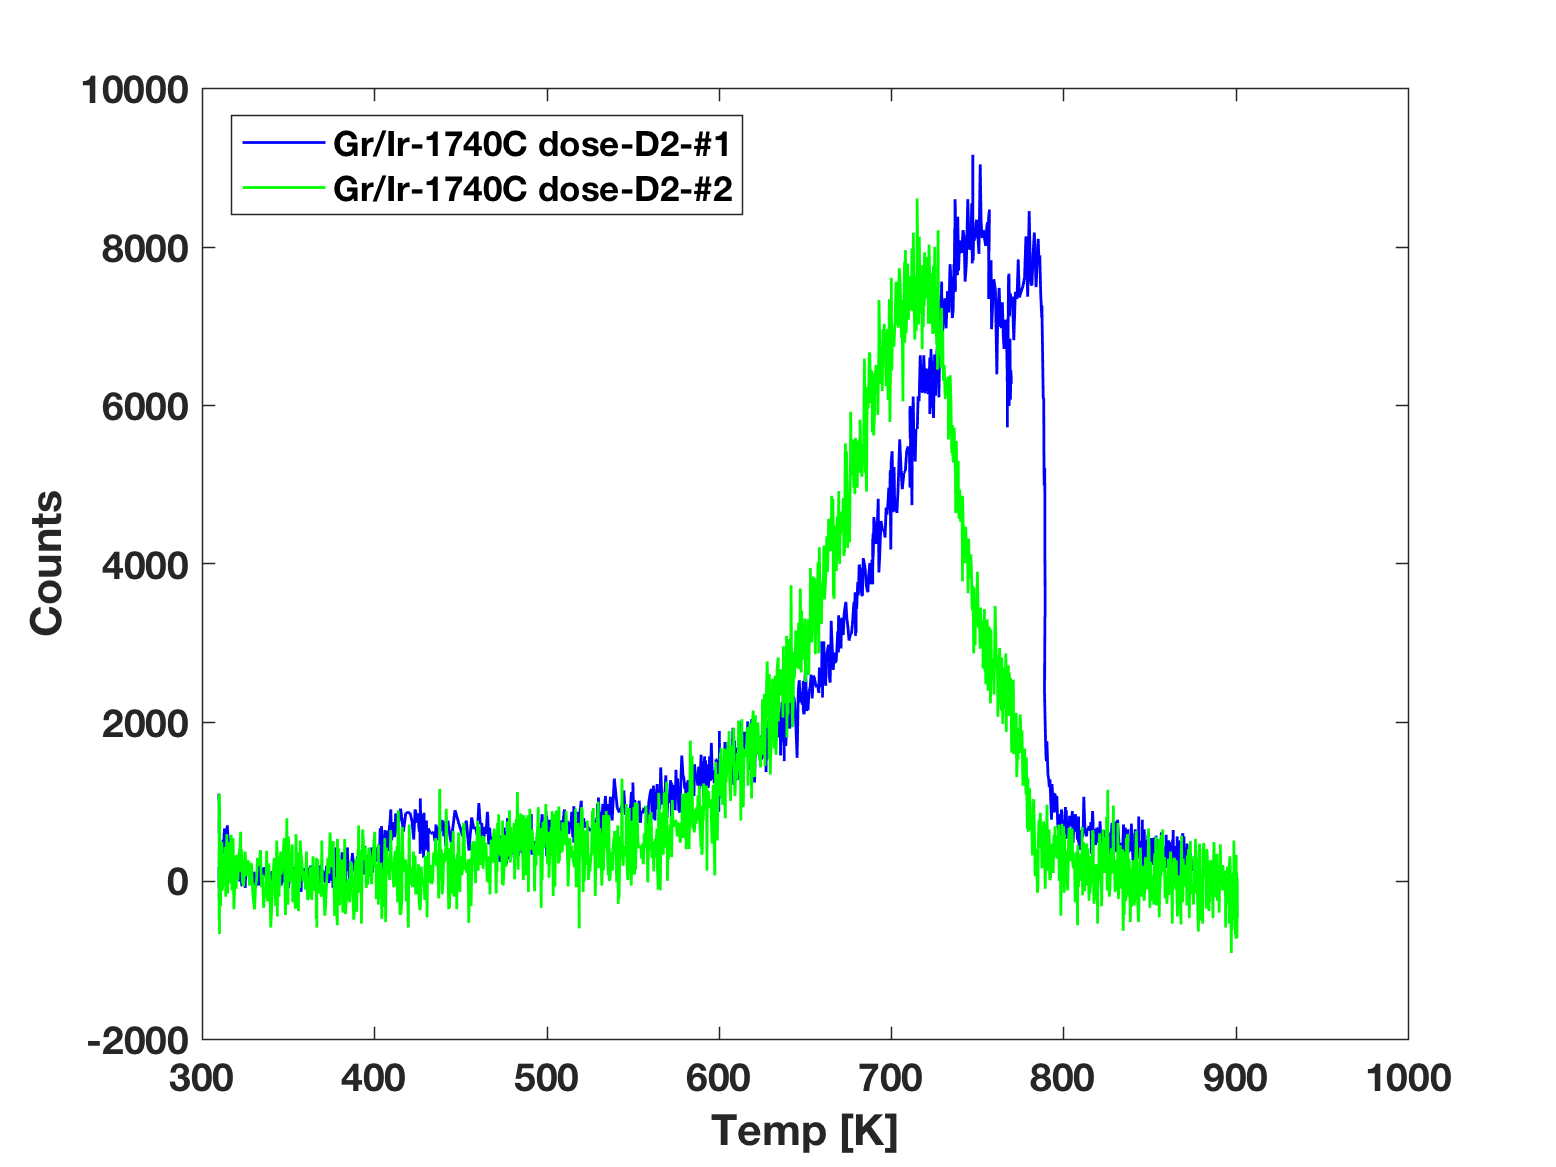
\includegraphics[width=\textwidth]{TPD/050516IrSorenD2dose1hourtemp.png}
    \caption{TPD of Gr/Ir after 1 hour dose of D$_2$ with a doser temperature of 1740 \degree C.}
    \label{TPD:D2}
  \end{subfigure}\hspace{0.5cm}
  \begin{subfigure}[b]{0.45\textwidth}
    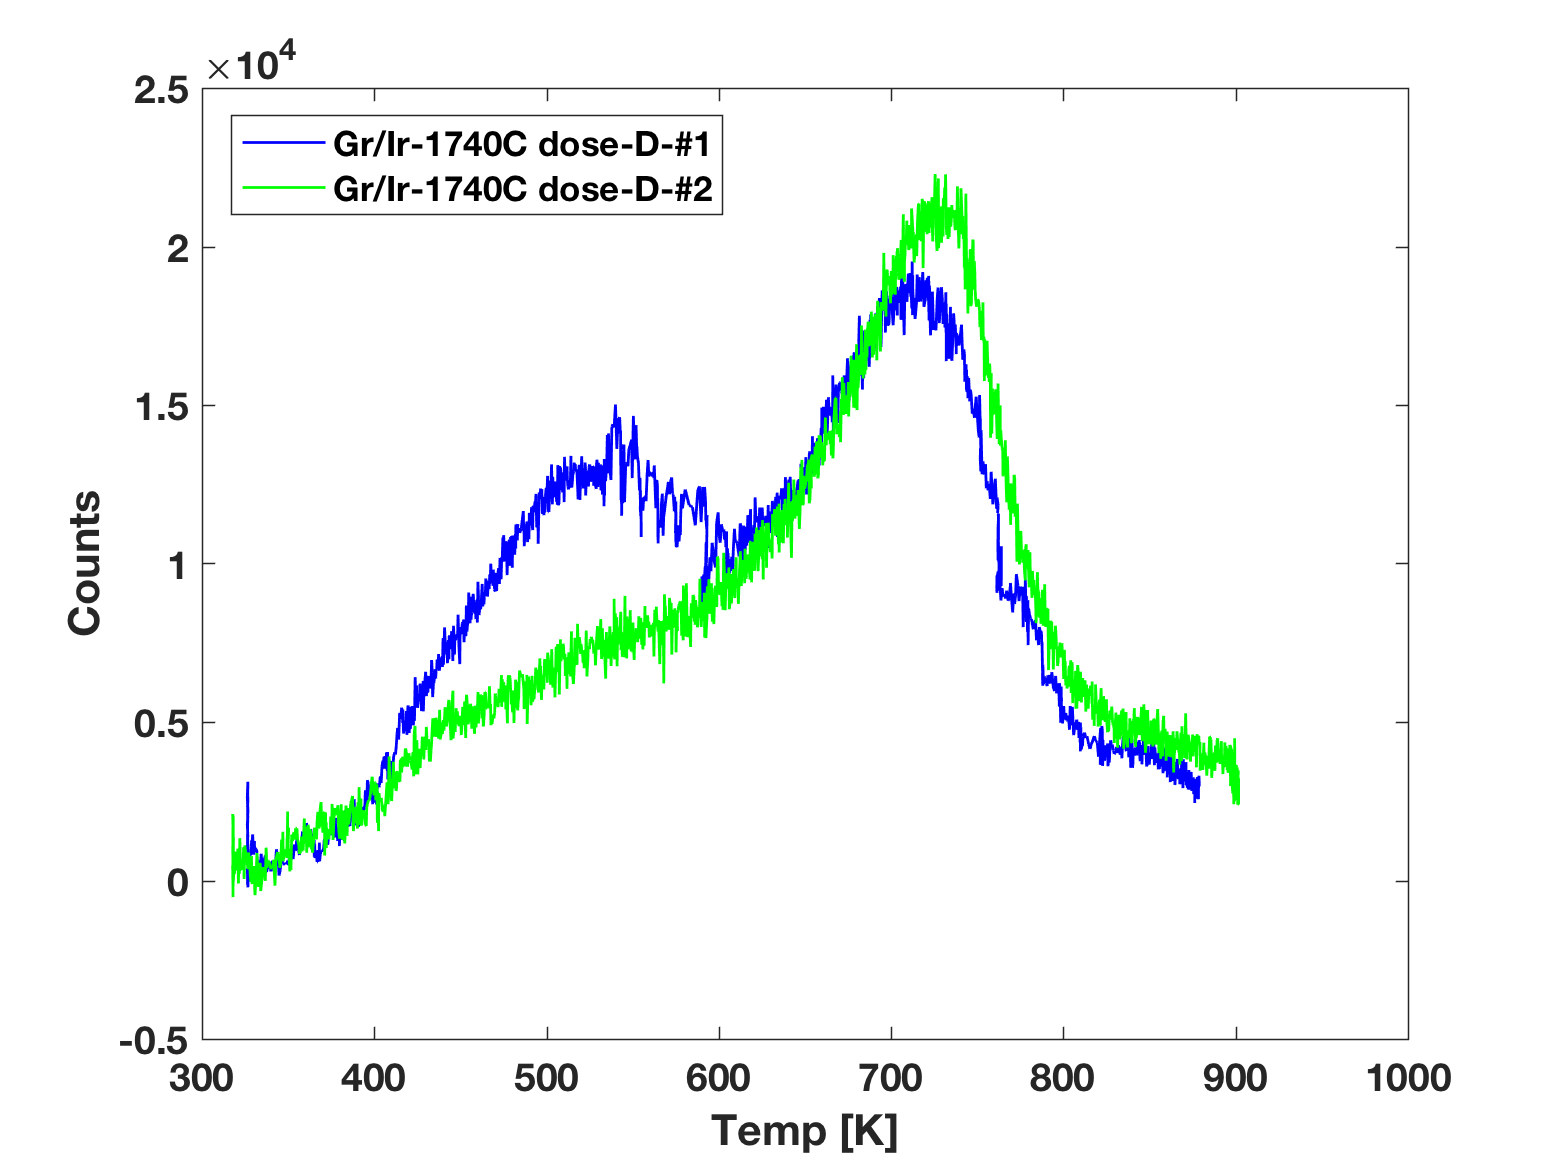
\includegraphics[width=\textwidth]{TPD/050516IrSorenDdose1hourtemp.png}
    \caption{TPD of Gr/Ir after 1 hour dose of atomic deuterium with a doser temperature of 1740 \degree C.}
    \label{TPD:D}
  \end{subfigure}
  \caption{}
  \label{TPD:all}
\end{figure}


\begin{figure}[H]
  \centering
  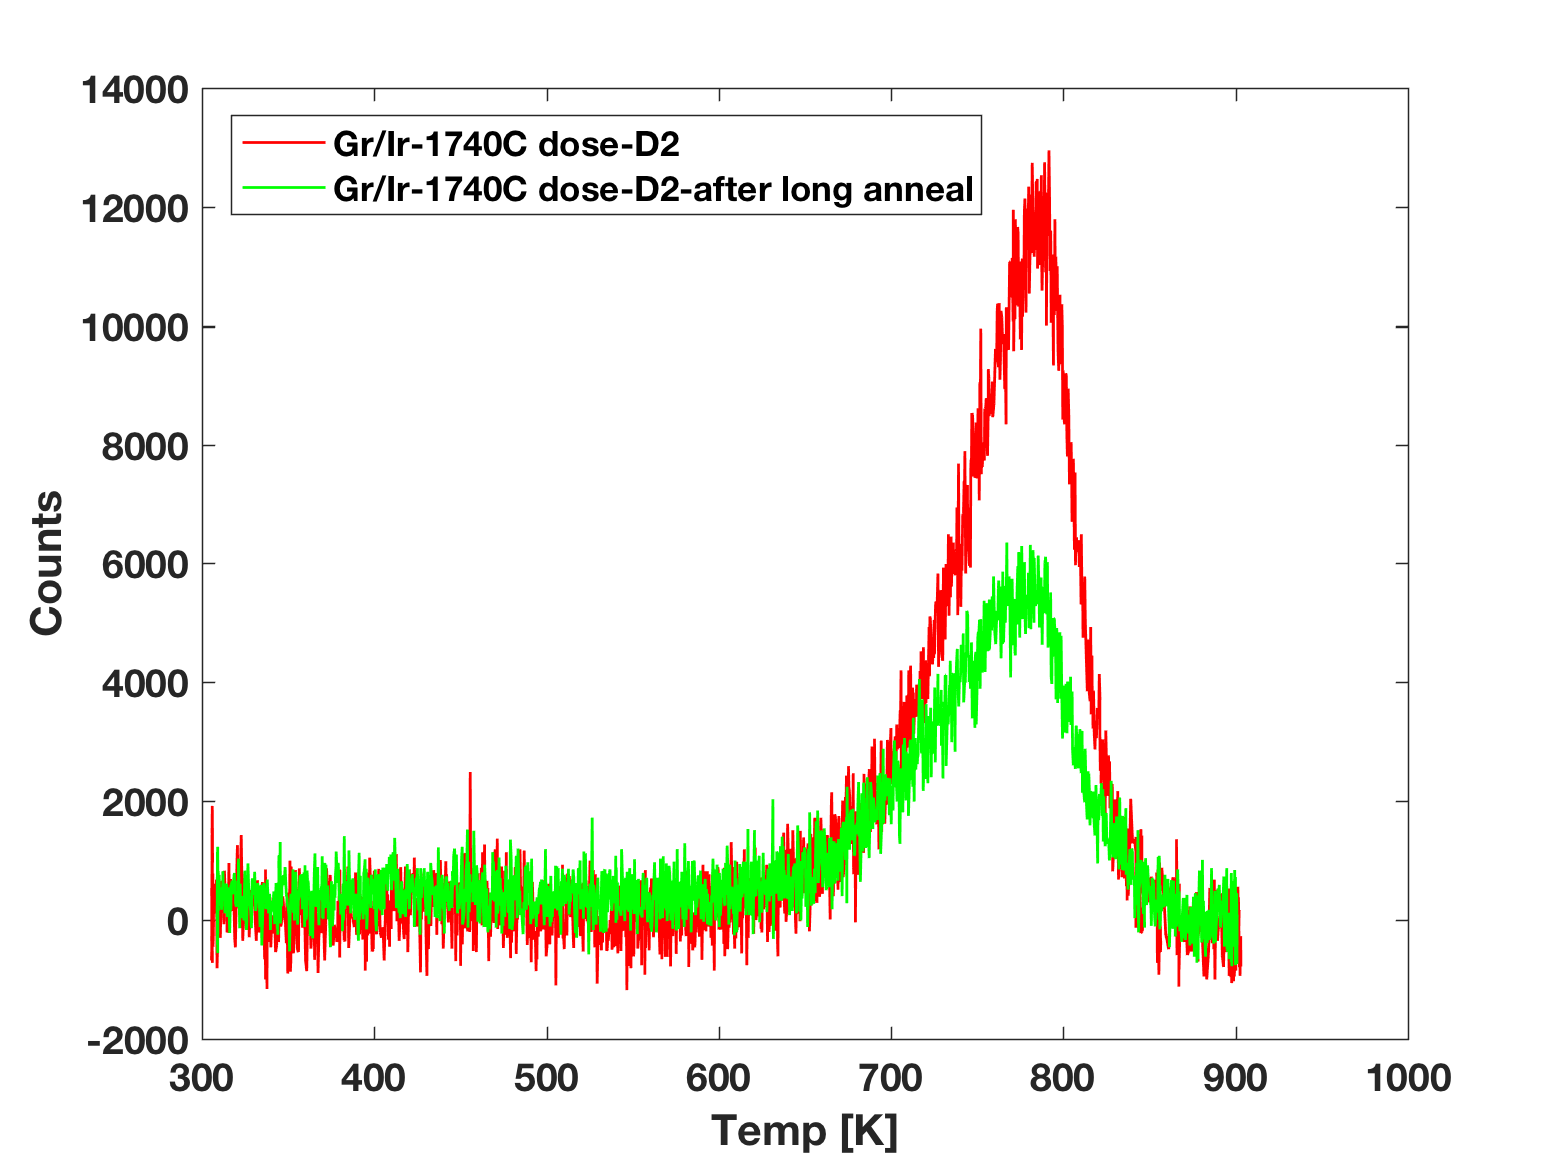
\includegraphics[width=0.6\textwidth]{TPD/GrIr1740CD2longannealtemp.png}
  \caption{}
  \label{TPD:bilayer}
\end{figure}
\section{Bilayered graphene on Ir}


\section{LEED of bilayered sample}

\begin{figure}[H]
\makebox[\textwidth][c]{
  \begin{subfigure}[b]{0.3\paperwidth}
    \includegraphics[height=\textwidth]{LEED/No" "flash/145eV.JPG}
    \caption{LEED without flashing. 145eV}
    \label{}
  \end{subfigure}
  \begin{subfigure}[b]{0.3\paperwidth}
    \includegraphics[height=\textwidth]{LEED/Low" "T" "flash/145eV.JPG}
    \caption{LEED after low temperature flash of the sample. 145eV}
    \label{}
  \end{subfigure}
  \begin{subfigure}[b]{0.3\paperwidth}
    \includegraphics[height=\textwidth]{LEED/post" "1090" "flash/145eV.JPG}
    \caption{LEED after high temperature flash. 145eV}
    \label{}
  \end{subfigure}
}
\caption{}
\label{}
\end{figure}

\chapter{Conclusion and future perspectives}

\section{conclusion and future perspectives}
Hydrogenation of graphene on Ir(111) by using vibrationally excited molecules has been investigated throughout this project. Pure graphene on Ir(111) was initially investigated along with the defects by carbon vacancies. The moiré pattern arising from graphene on Ir(111) has been observed by using STM. Hydrogenation by vibrationally excited molecules was proven successful and the influence of the flux of atomic hydrogen has been investigated. This was done by scanning the hydrogenated surface following doses with the atomic beam source at temperatures of 1745\degree C, 1593 \degree C, and 1343\degree C. Having a D$_2$ chamber pressure of $5 \cdot 10^{-7}$mbar during dosing, it was found that hydrogen coverages of after 20 min doses were; 35\%, 28\%, and a few \%.\\
TPD measurements revealed that hydrogen dimers only form after hydrogenation by atomic hydrogen. Furthermore it was calculated from the TPD measurements that hydrogen on graphene on Ir(111) in the HCP and FCC sites has an energy of desorption around 2.0-2.1$\pm$0.41eV. \\
\\
Her mangler stadig noget. Blandt andet hvilke eksperimenter der ville være relevante hvis der var mere tid.

\appendix
\chapter{Additional figures} \label{App:A}


%%%%% BIBLIOGRAPHY %%%%%
\nocite{*}
\bibliographystyle{unsrt}
\bibliography{references}
\end{document}
